\documentclass{beamer}
\usetheme{Madrid}
\usefonttheme[onlymath]{serif}
\usepackage{multicol}
\usepackage{graphicx}
\usepackage{hyperref}
\usepackage{amssymb}
\usepackage{tcolorbox}
\usepackage{listings}
\usepackage{float}
\usepackage{tikz}
\usetikzlibrary{positioning,decorations.pathreplacing,shapes}
\author{Harry LaBollita}
\institute{Arizona State University}
\title{Kinetic Folder Update}
\date{February 12, 2020}
\logo{
\includegraphics[scale =0.2]{asu.png}}
\setbeamertemplate{navigation symbols}{}
\setbeamertemplate{title page}[default][colsep=-4bp,rounded=true]
\definecolor{asu_maroon}{HTML}{8C1D40}
\definecolor{asu_gold}{HTML}{FFC627}
\setbeamercolor{palette primary}{bg=white, fg=black}
\setbeamercolor{title}{fg=black}
\setbeamercolor{frametitle}{fg=black}
\setbeamercolor{itemize item}{fg=black, bg = black}
\setbeamercolor*{author in head/foot}{bg = asu_gold, fg = asu_maroon}
\setbeamercolor*{title in head/foot}{bg = asu_gold, fg = asu_maroon}
\setbeamercolor*{date in head/foot}{bg = asu_gold, fg = asu_maroon}
\setbeamertemplate{itemize items}[default]
\setbeamertemplate{enumerate items}[square]
\setbeamercolor{itemize items}{bg =asu_maroon, fg=asu_maroon}
\setbeamercolor{item projected}{bg =asu_maroon, fg=white}


\begin{document}

\frame{\titlepage}

\begin{frame}{"Bad Seq" Dataset}

\begin{itemize}
\item 117 sequences
\item Variable length (max: 80 ntds)
\end{itemize}
\begin{table}
\centering
\begin{tabular}{|ccc|}
\hline
{\bf Stats} & {\bf Kinetic Folder} & {\bf viennaRNA}\\
\hline
\hline
{\bf Mean} & 0.48 & 0.37 \\
{\bf Best} & 0.30 & 0.25 \\
{\bf Worst} & 0.62 & 0.53\\
\hline
\end{tabular}
\end{table}
\end{frame}

\begin{frame}{Results}
\begin{figure}[H]
\centering
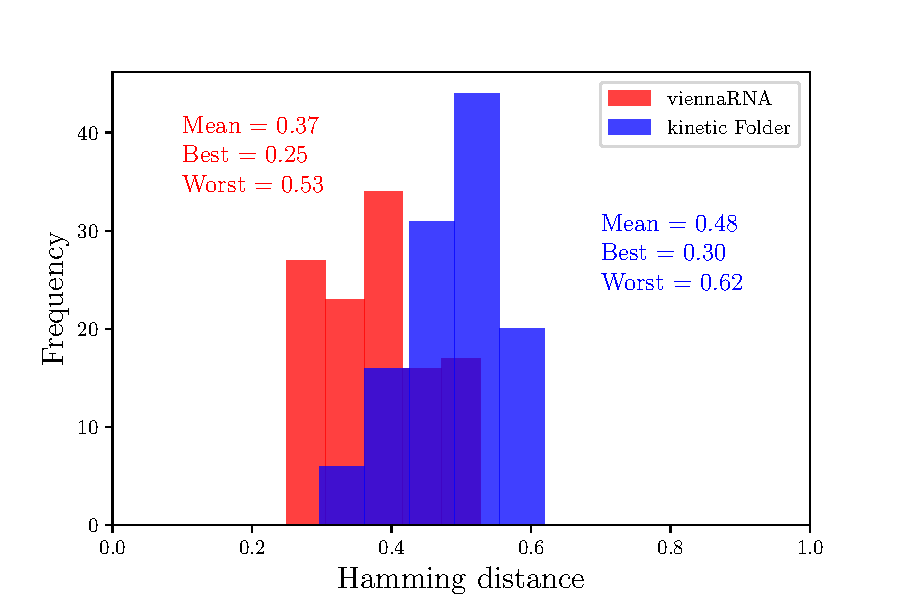
\includegraphics[scale =0.625]{bad_seq_plot.pdf}
\end{figure}
\end{frame}

\subsection*{Pseudoknotted dataset}
\begin{frame}{pseudoknotted}
\begin{itemize}
\item 15 sequences with pseudoknotted secondary structures\footnote{Sequences from \href{http://pseudobaseplusplus.utep.edu}{Pseudobase++} }
\item Mean length: 29 ntds
\end{itemize}
\begin{table}
\centering
\begin{tabular}{|ccc|}
\hline
{\bf Stats} & {\bf Kinetic Folder} & {\bf viennaRNA}\\
\hline
\hline
{\bf Mean} & 0.48 & 0.35 \\
{\bf Best} & 0.29 & 0.25 \\
{\bf Worst} & 0.77 & 0.62\\
\hline
\end{tabular}
\end{table}
\end{frame}

\begin{frame}{Results}
\begin{figure}
\centering
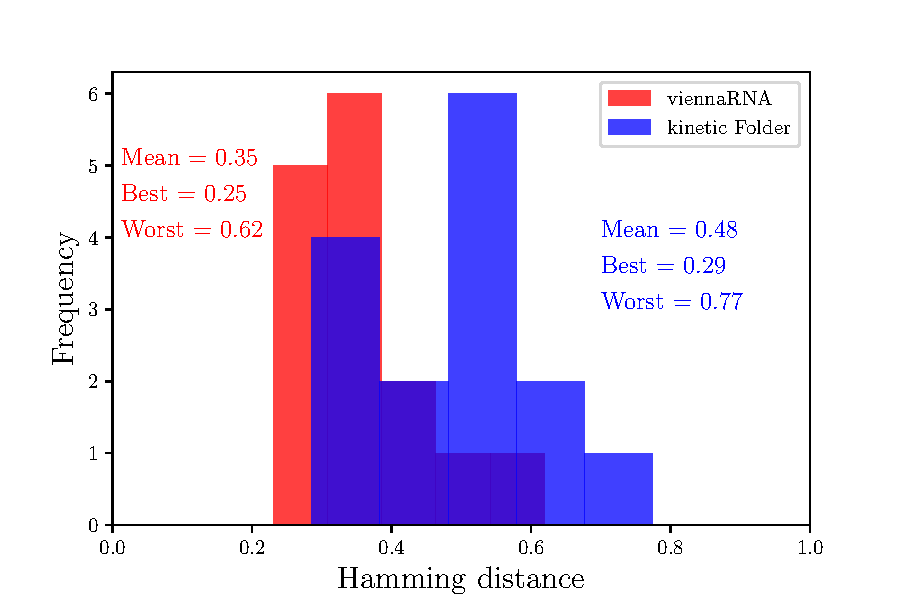
\includegraphics[scale=0.625]{pseudo_plot.pdf}
\end{figure}
\end{frame}

\section*{Mapping function}
\begin{frame}{Mapping function}
A schematic of where the mapping function $\mathcal{M}(\mathcal{S})$ will be implemented in the roll-out algorithm.
\begin{figure}
\centering
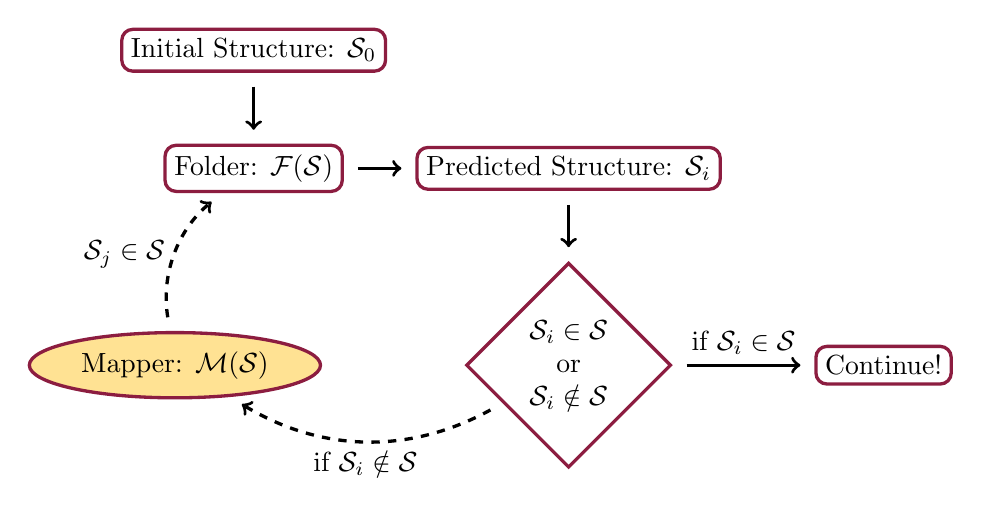
\begin{tikzpicture}
\node (S0) [rectangle, rounded corners, draw = asu_maroon, very thick, text centered] at (0,4) {Initial Structure: $\mathcal{S}_{0}$};
\node (Folder) [rectangle, rounded corners, draw = asu_maroon, very thick, text centered] at (0, 2.5) {Folder: $\mathcal{F}(\mathcal{S})$};
\path [->, shorten <=5pt, shorten >=5pt, very thick] (S0) edge (Folder);
\node (Si) [rectangle, rounded corners, draw = asu_maroon, very thick, align = center] at (4, 2.5) {Predicted Structure: $\mathcal{S}_{i}$};
\path [->, shorten <=5pt, shorten >=5pt, very thick] (Folder) edge (Si);
\node (Q) [diamond, draw = asu_maroon, very thick, align = center] at (4,0) {$\mathcal{S}_{i} \in \mathcal{S}$\\or\\$\mathcal{S}_{i} \notin \mathcal{S}$};
\path [->, shorten <=5pt, shorten >=5pt, very thick] (Si) edge (Q);
\node (Map) [ellipse, draw = asu_maroon, very thick, text centered, fill = asu_gold!50] at (-1, 0) {Mapper: $\mathcal{M}(\mathcal{S})$};
\node (Finish) [rectangle, rounded corners, draw = asu_maroon, very thick, text centered] at (8,0) {Continue!};
\path [->, shorten <=5pt, shorten >=5pt, very thick] (Q) edge node[above] {if $\mathcal{S}_{i} \in \mathcal{S}$}(Finish);
\path [->, dashed, shorten <=5pt, shorten >=5pt, very thick, bend left] (Q) edge node[below] {if $\mathcal{S}_{i} \notin \mathcal{S}$}(Map);
\path [->, dashed, shorten <=5pt, shorten >=5pt, very thick, bend left] (Map) edge node[left] {$\mathcal{S}_{j} \in \mathcal{S}$}(Folder);
\end{tikzpicture}
\end{figure}
\end{frame}

\begin{frame}[fragile]{Mapping function}
\framesubtitle{Example from Folder}
\begin{tcolorbox}[colframe = asu_maroon, colback = white, title = Output of Kinetic Folder]
\begin{verbatim}
+:[[3,17],[4,16],[5,15]]...(((.........)))........
+:[[10,21],[11,20],[12,19]]...(((....[[[..))).]]].....
-:[[3,17],[4,16],[5,15]]..........(((......)))........
+:[[3,17],[4,16],[5,15],[6,14]]...((((...[[[.)))).]]]...
\end{verbatim}
\end{tcolorbox}
\end{frame}
\end{document}
